\section{METHODS}

 The system used for all experiments consists of a carefully selected set of hardware, sofware, and materials.

For our tendons, we use [@victor material] strings instead of string or wire, so they are less prone to damage from wetting in cadaveric experiments, and so the wire stress extension is minimal.

 Two identical systems were designed, one to be used primarily for cadaveric experiments (wet lab) and another for exclusively non-biological specimens (dry lab).

\\subsection{FPGA Controller implementation} % (fold)
\label{sub:fpga_controller_implementation}
An FPGA is a field-programmable gate array- a small circuit which can represent functions as circuit implementations.
We opted to use FPGA in exploring these points:
\item FPGA's run in a deterministic time, and thus their latencies are several orders of magnitude faster than even an optimized CPU implementation. We have the opportunity to set the clock timing to exactly the rate we want, while GPU procesing could become lagged.
\item With consistent clock frequency being of paramount importance, the FPGA has low-variance in delivering results, becuase it's powered by an independent hardware timer that's dedicated to the FPGA.

FPGA Card (NI PXI-7952R FlexRIO)
DAQ Card (NI PXI-625X)
Timing I/O Card (NI PXI-6602) - Receives the encoder pulses, and receives the pulses per second to 
DC Motor, Encoder, Gear Head  (Faulhaber 3883H024C+HEDS5500A12 + X074343)
PXI Chassis (NI PXI-104x )
Embedded Controller + CPU (NI PXI-8108)




We used a PXI Bus to handle the direct memory acess between the FPGA IO buffers and the DAQ (NI PXI-625X).


\begin{figure}[schematic_finger_overhead]
  \label{fig:schematic_finger_overhead}
  \centering
  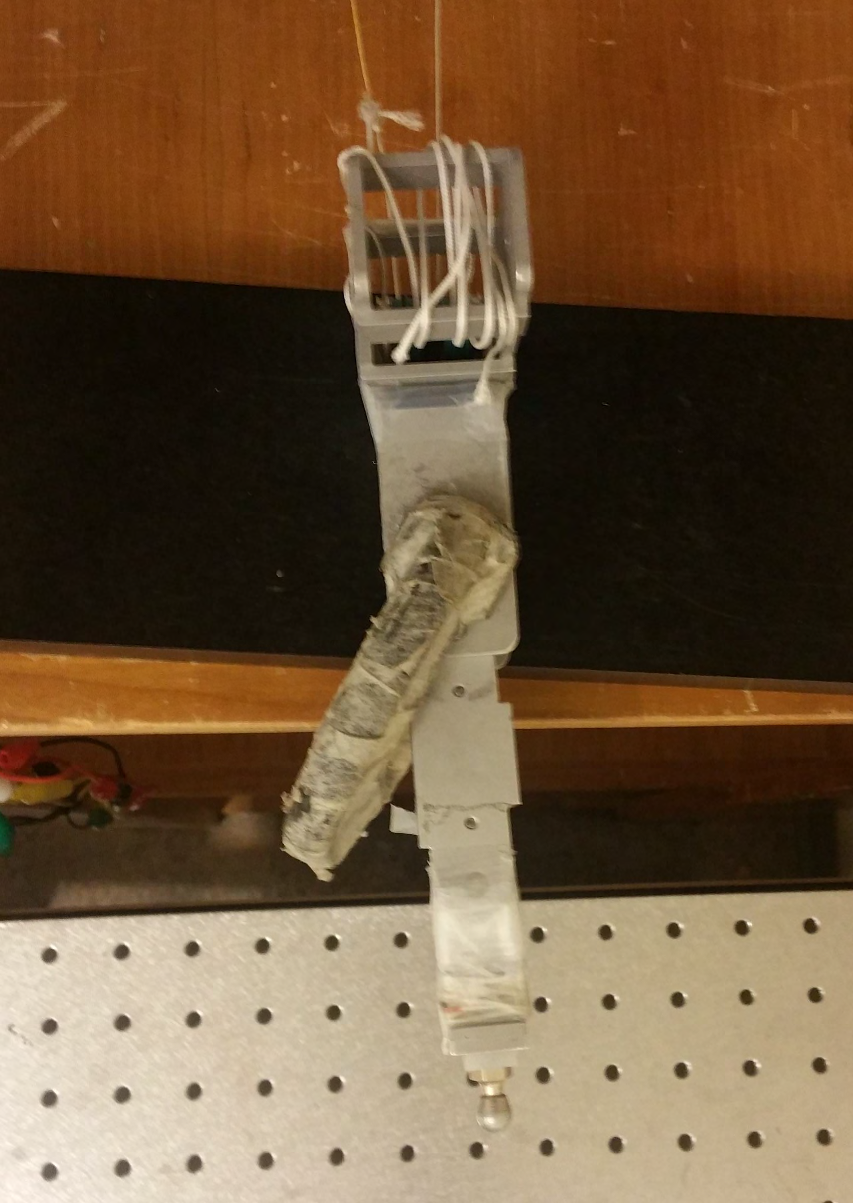
\includegraphics[width=0.5\textwidth]{figures/overhead_robotic_finger.pdf}
  \caption{Tendon driven robotic finger with one joint, 1DOF, 2 muscles}
\end{figure}

\begin{figure}[hardware_schematic]
  \label{fig:hardware_schematic}
  \centering
  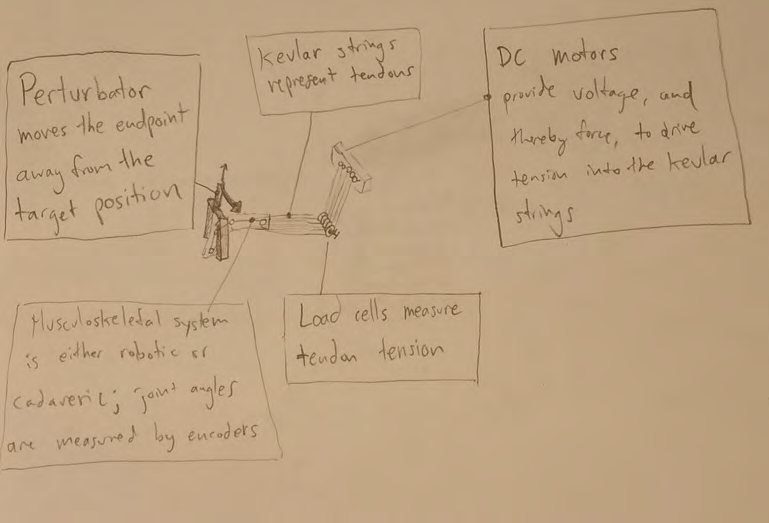
\includegraphics[width=1.0\textwidth]{figures/hardware_schematic.pdf}
  \caption{Caption one two three}
\end{figure}

\begin{figure}[fpga_schematic]
  \label{fig:fpga_schematic}
  \centering
  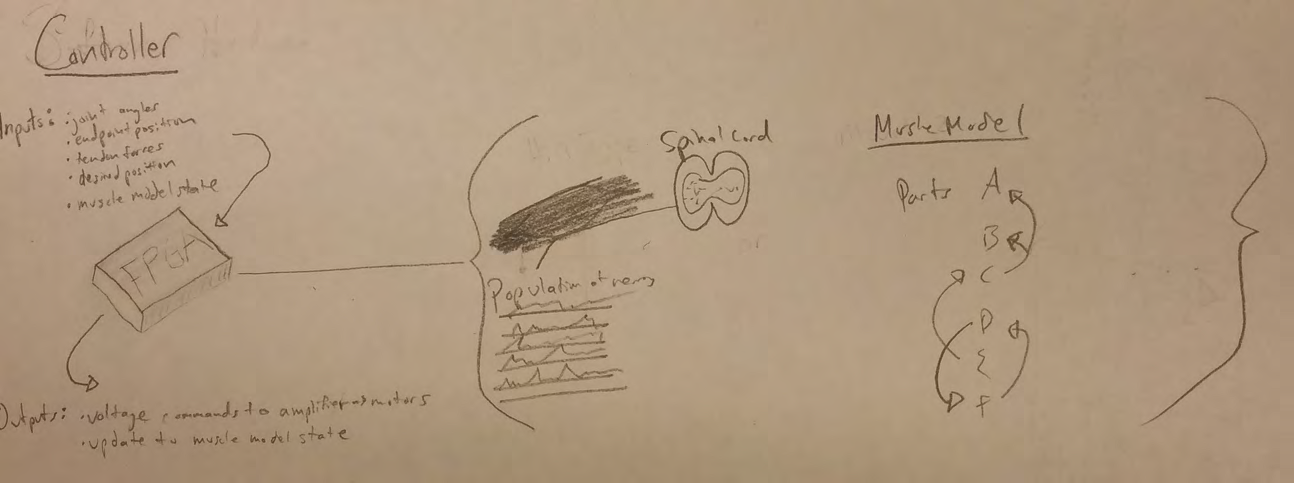
\includegraphics[width=1.0\textwidth]{figures/fpga_schematic.pdf}
  \caption{Caption one two three}
\end{figure}


\begin{figure}[loadcells_pulley]
  \label{fig:loadcells_pulley}
  \centering
  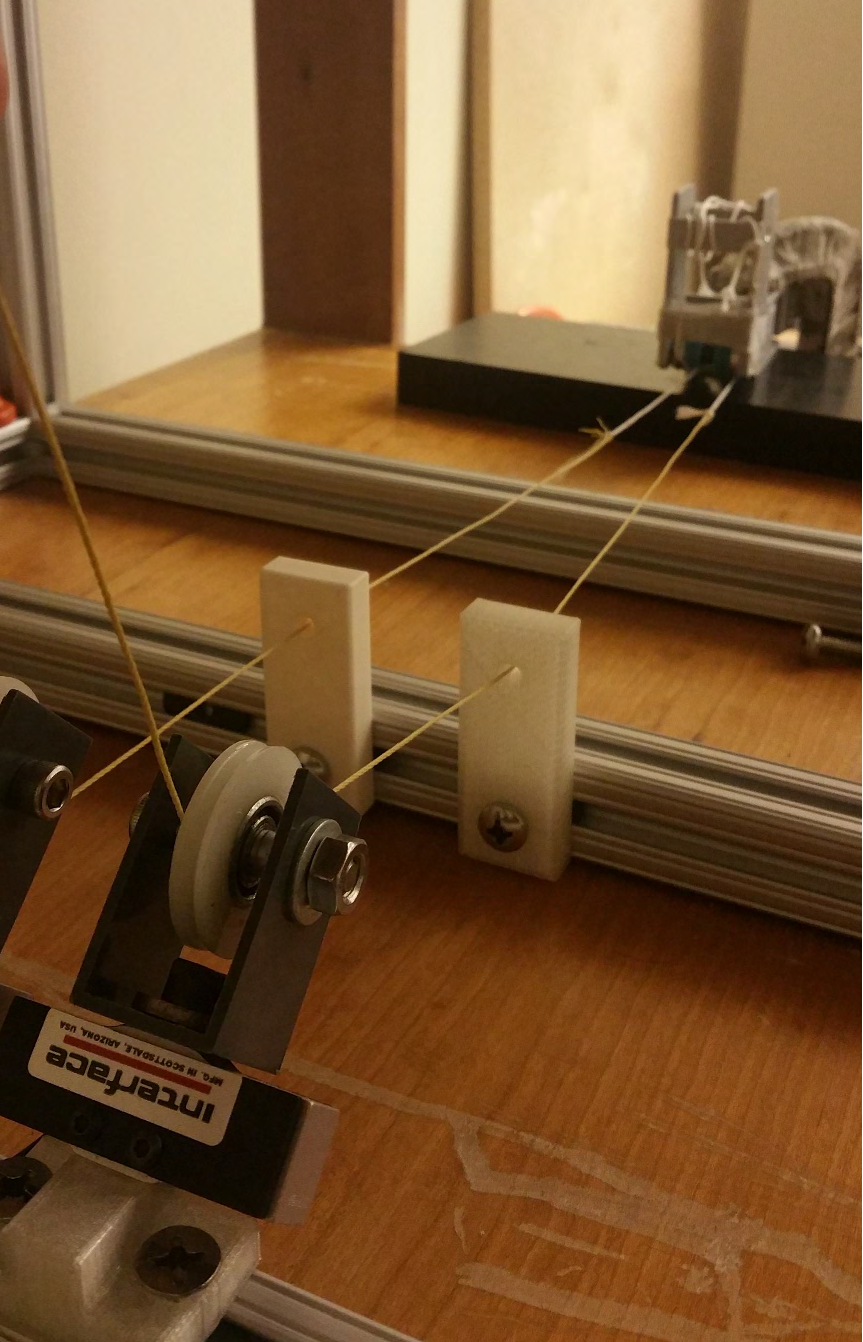
\includegraphics[width=0.5\textwidth]{figures/loadcells_pulley.pdf}
  \caption{Caption one two three}
\end{figure}
\begin{figure}[motor_closeup]
  \label{fig:motor_closeup}
  \centering
  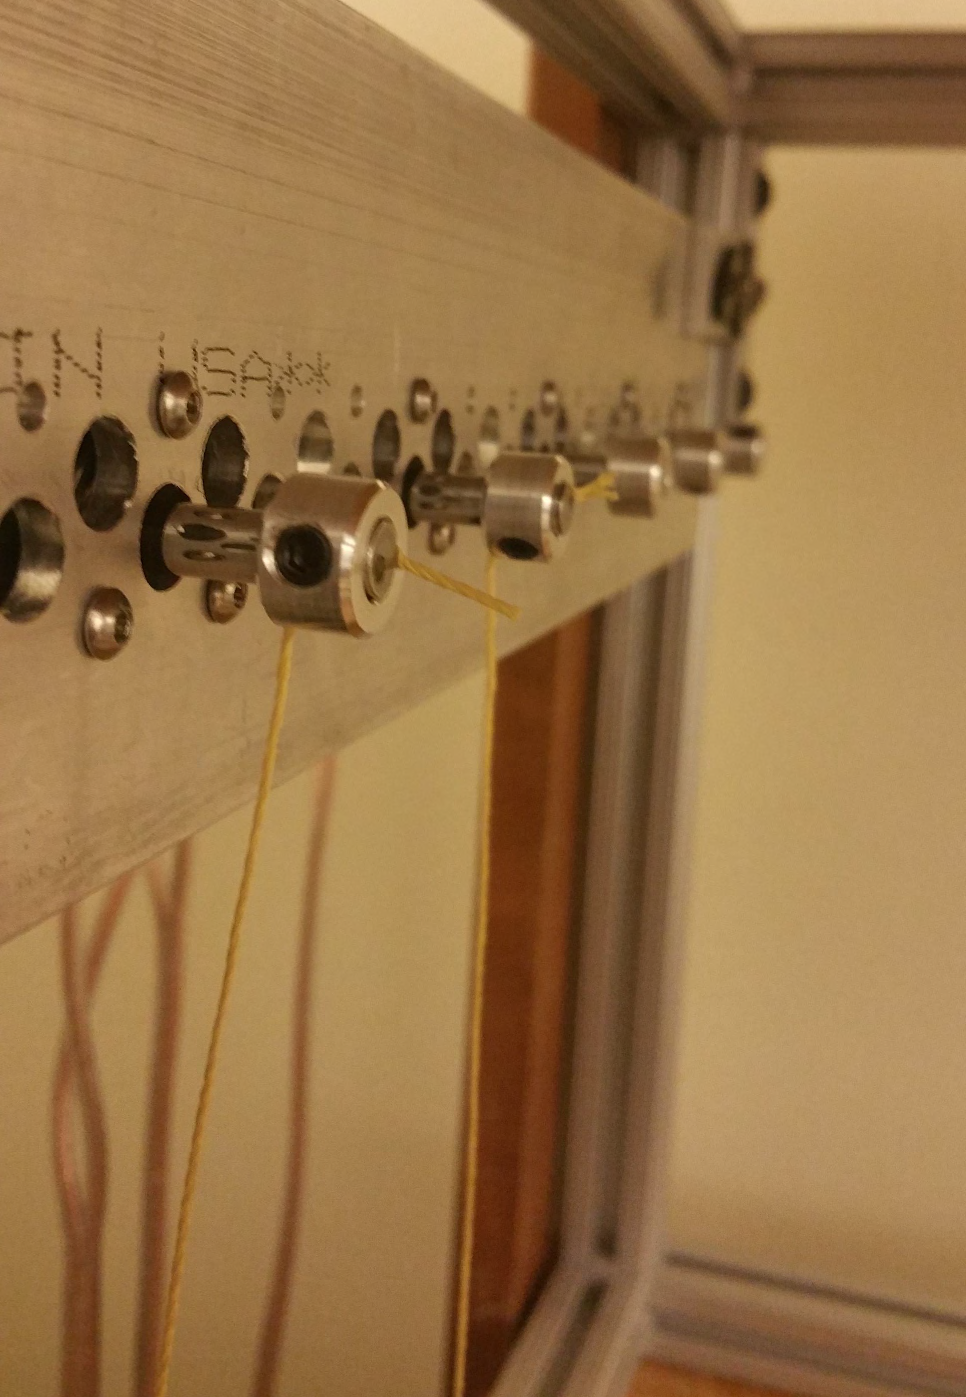
\includegraphics[width=0.5\textwidth]{figures/motor_closeup.pdf}
  \caption{Caption one two three}
\end{figure}
